\documentclass{sig-alternate}
\usepackage{url}
\usepackage{verbatim}
\usepackage[utf8]{inputenc}
\usepackage{microtype}
\usepackage{booktabs}
\usepackage{upquote}
\usepackage{url}
\usepackage{algpseudocode}
\usepackage{algorithm}


%\hyphenation{brow-ser brow-sers tra-dit-ion-al ja-va-script Web-Kit}
\begin{document}
\CopyrightYear{2013}
\clubpenalty=10000
\widowpenalty=10000

\title{Measuring Server-side Compliance of Do Not Track}
\numberofauthors{2}
\author{
\alignauthor
Yuze Lang\\
      \affaddr{Carnegie Mellon University}\\
      \affaddr{ylang@andrew.cmu.edu}
\alignauthor
Ruoyu Li\\
      \affaddr{Carnegie Mellon University}\\
      \affaddr{ruoyul@andrew.cmu.edu}
}

\newcommand{\todo}[1]{\textbf{[TODO: #1]}}

\maketitle
\begin{abstract}
Do Not Track header is proposed for expressing unwillingness for a web user to be tracked and requesting a web application disable its tracking for the individual user.
\end{abstract}

\terms{Privacy}

\keywords{DNT, Third Party Tracking, Online Behavioral Advertising}

\section{Introduction}\label{sec:intro}
Online behavioral advertising (OBA)~\cite{sheltononline} is a type of targeted advertising, by which companies track consumers’ online activities to target them for digital advertising directed at their specific interests. Web users could easily see targeted advertisement in embedded block on their browsing websites because of this technique. For instance, a user might able to see several advertisement about "cheap flight to Italy" after searching on search engine with key work "european trip" and visited several results listed. This is because when the user visit several websites contains DOM element which will send HTTP request to third party tracker. By reading and setting cookie, the third party tracker will be able to track the user's browser history, thus classify the user with interests.

This technique seems to be beneficial for both advertisement publishers and advertisement platform, since publishers are able to push their advertisements to fewer but more accurate targets, and advertisement platform, who has the ability to classify targets, will attract more publishers to use their network. It even might be non-harmful since ideally, users are supposed to see those advertisements that is helpful for them specifically. However, privacy concern could be raised. Web users are being tracked: their browsing history is logged into third party companies' database without any awareness. Their interests, hobbies, even recent plans would be released to those trackers. This kind of tracking is blind to the willingness of users. I.e., when if the user does not want to be tracked, unless to reject all third party cookies, there is no good way to disallow the tracker.

The concept of \emph{Do Not Track} (DNT)~\cite{tschofenignot} was firstly proposed and prototyped in 2009 by researcher Christopher Soghoian, Sid Stamm, and Dan Kaminsky on Firefox web browser~\cite{wikidnt}. DNT is proposed to be an HTTP request header in HTTP request header field send along HTTP requests. It is a protocol that presents the unwillingness of the user to be tracked. Ideally, it requests that a web application disable either its tracking or cross-site user tracking of an individual user.

Due to the concept of \emph{Do Not Track} and its implementation, there are no technical enforcement mechanisms built-in~\cite{tschofenignot}. Thus there is the question of how users (or more realistically researchers, etc. on behalf of users) detect success or failure to comply. A research project in Carnegie Mellon University did a study on privacy protection tools~\cite{balebako2012measuring}. In this study, Do Not Track has been considered as a way to limit behavioral advertising and the measurement on Do Not Track is done by their methodology. The basic idea is to first generated browsing history on a topic key word with and without DNT header, and then browse the website that contains online behavioral advertising. To compare the similarity between the advertisement showed up and the key word, the effectiveness of privacy tool is revealed.

Our study here is inspired by this project and the research paper \emph{Measuring the effectiveness of privacy tools for limiting behavioral advertising}~\cite{balebako2012measuring} written by Lorrie Faith Cranor \emph{et al}. We did a study on the protocol Do Not Track and research by Lorrie \emph{et al}, learned some takeaway and then attempted to measuring the effectiveness of Do Not Track specifically. Here, measuring the effectiveness of Do Not Track is more meaningful to measuring the server-side compliance of Do Not Track, since in the current stage, the web services and networks who claimed to support DNT is limited. To test on those services who does not support DNT is meaningless, and the result would be able to anticipated easily.

We did an experiment similar to the experiment in the study of Lorrie \emph{et al} targeting on DNT supported network services. We exposed more issues and problems both regrading to the Do Not Track itself, and the study. The value of this paper is not limited to a measurement of Do Not Track on companies who claimed to respect Do Not Track, but also revealed several issues and problems on the concept of Do Not Track itself and the methodology of detect success or failure to comply.

In this paper, we introduce the Do Not Track concept, present our experiment methodology and results, and talked about the limitations. The limitations includes the design limitation of the concept, and mainly on the methodology of Lorrie's study and ours. Because of this is a project limited within a course background, we are limited in budget and time. Due to the fact both Do Not Track, which is still in draft stage, and our target sites are updated frequently, results and thesis in this paper is updated up to the current. We anticipate that it could be out of date if the concept of Do Not Track changes.

\paragraph{Organization}
The rest of this paper is organized as follows. Section~\ref{sec:background} presents some basic concepts related to the study.  Section~\ref{sec:lorrie} describes the Lorrie \emph{et al}'s study, which inspires our research. Section~\ref{sec:services} states the companies who supports Do Not Track. Section~\ref{sec:experiment} describes our experiment procedure. Section~\ref{sec:limitation} discusses some limitation in the study. Section~\ref{sec:conclusion} concludes.

\section{Background} \label{sec:background}

In this section, we would like introduce in detail about several background concepts and knowledges, including \emph{Online Behavioral Tracking}, \emph{Online Behavioral Advertising} and \emph{Do Not Track}. 
\subsection*{Online Behavioral Tracking}

Third-party tracking is used for a lot of purposes on the web. While it can be beneficial for third party to track a user to provide more useful content such as social integration and personalized content, it can also be used to track a user’s browsing history across the internet which can then be used for advertising purposes. 

When a user visit a first party webpage, if some third party content is embedded in the page, the third party will get a HTTP request from the user as well, requesting the embedded content from the third party. The third party is then able to set a cookie in the user’s browser and access information on the page of first party (such as by looking at the HTTP referrer, or getting the document.title if the embedded element is a script; some first party might even voluntarily shares the data to a third party). 

Besides tracking the users with HTTP cookie, there are many other ways by which a third party can track a user. In the paper Third-Party Web Tracking: Policy and Technology~\cite{mayer2012third}, Mayer and Mitchell talks about many other technologies to pseudonymously track the user. For example, there are stateful tracking technology such as HTTP cache ETags, TLS/SSL session ID, HTML5 storage, and stateless fingerprinting such as IP address, user agent, and operating system. A combination of these technologies can be used to uniquely identify a user across the web even if no HTTP cookies are used. The paper also cites a 2010 study by Eckersley that reports 83.6\%browsers out of 500,000 were uniquely identified with a subset of active fingering features. This has an implication on the effect of DNT if it works and all servers respect the header: DNT will be more effective than the methods that only deals with rejecting third party cookies since the compliant servers will stop using all means to stop tracking the user; furthermore, DNT will have the benefit of not breaking a lot of features on the web such as social integration since the DNT specification~\cite{tracking_compliance_20130430} allows necessary gathering of data to perform essential functionalities under some constraint. 

The browsing history a third-party already reveals enough information about a user to raise serious concerns for both the users and policy makers. To make the matter worse, there are means through which a tracking company can obtain identifiable data about a user making the tracking no longer anonymous or even pseudonymous. According to a post on Stanford CIS blog titled There is No Such Thing as Anonymous Online Tracking~\cite{nosuchthing}, there are mainly 5 ways a third party can get data that able to personally identify a user. The primary way is when a third party is also a first party in another context, where the users voluntarily provide their identity. For example when a Facebook user visits another websites page, Facebook is able to tell where the user has been if the other page embeds Facebook widgets such as like button or comment box. Facebook is then able to provide a better targeted ad to the user with this learned browsing history. A second way, as we have talked about, is that a first party might voluntarily provide its users’ identity, if the two parties are cooperating or if the first party is selling the data for pay. Third, a first party may unintentionally leak identity such as by appending the user id after the user’s profile page. Additionally, a third party can obtain identifiable information by exploiting a first-party security vulnerability or matching pseudonymous browsing histories against identified datasets. 

As we can see from above, third party tracking can reveal much information about a user including his/her browsing history, general interest, purchases, employment status and much more even including personally identifiable information. This is the reason why there has been much discussion on third-party tracking and DNT as a way to limit tracking to protect the user’s privacy.

\subsection*{Online Behavioral Advertising}

\todo{ruoyul: add OBA}

\subsection*{Do Not Track}

Do Not Track is a combination of technology and policy attempt to enable users to opt out of third party tracking. It is a header field in the user’s HTTP request sent from the browser. The receiving web application/server of the HTTP request with DNT turn on is expected to cease tracking the user and not use the data stored in user agents. The Do Not Track header was originally proposed in 2009 by researchers Christopher Soghoian, Sid Stamm, and Dan Kaminsky. It is currently being standardized by the W3C~\cite{wikidnt}, and supported by most mainstream browsers. 

The header field name is DNT and it currently accepts three values: 1 in case the user does not want to be tracked (opt out), 0 in case the user consents to being tracked (opt in), or null (no header sent) if the user has not expressed a preference. The default behavior is not to send the header, until the user chooses to enable the setting via their browser~\cite{wikidnt}. 

The approach of DNT has a couple of benefits. First of all, the way of sending a HTTP header is completely compatible with the existing web technology. No large amount of additional work needs to be done at the server side to support DNT so that the existing internet ecosystem is not broken. Similarly, only a small amount of work is needed on the user agent to support sending the header. The user does not need to do anything such as installing a plugin or setup the browser so that adoption should be easier.

Second of all, although some advertising companies allow user to opt of tracking by providing their own page to let the users specify their preference, there is no unifying and easy way to opt out of all companies that supports so. Furthermore, studies by McDonald and Cranor~\cite{mcdonald2010beliefs} and by Leon \emph{et al}.~\cite{leon2012johnny} suggests that the individual opt-out pages are not very effective and might be confusing to the users. Thus, DNT provide a easy and simple way for the user to express unwillingness to be tracked to all companies without adding much overhead.

\subsection*{Browser Behavior} \label{sec:browserbehavior}

Modern mainstream browsers are all supporting Do Not Track up to current. In Firefox 5 or later, user can set \emph{Tell websites I do not want to be tracked}, under privacy tab in preference setting, as enabled to automatically include \texttt{DNT} header in all HTTP requests. Similar settings are available on Chrome 23 or later, Opera 12 or later, and IE 9 or later. For Safari 5.1 or later, Do Not Track setting is hidden under \emph{Development} menu, which will show up only if user enables \emph{Show Develop menu in menu bar}.

After being set enabled to Do Not Track, browsers will include HTTP header \verb|DNT: 1| in all HTTP requests. According to \emph{The Web Tracking Protection} specification~\cite{w3cwtp}, DOM Property method of \verb|document.navigator.doNotTrack == "1"| must return \verb|TRUE|. This allows script to detect and respect user's preference to be not tracked. This feature is supported on Firefox 9 or later, IE 9 or later, Opera 12 or later and Safari 5.1 or later on OS X 10.7 or later. It is not supported by Chrome yet~\cite{navigatordnt}. Furthermore, IE 10 enables Do Not Track by default.~\cite{wikidnt}

\subsection*{Server-side compliance of Do Not Track}

Due to the fact that the design of Do Not Track protocol is a policy protocol rather than a technical limiting bond, compliance of Do Not Track is complicated and abstract. Only the general requirement is defined with no detailed technical specification. This is understandable since different services and networks might achieve the goal by various way. The compliance of a \emph{first party} and a \emph{third party} is different. In general first parties do not need to alter behavior with respect to the header except do not release information to third parties. Third party content elements are supposed to honor the header by declining to set cookies and record user activity on their servers~\cite{donotbeg}.

\paragraph{Compliance of First Party}

In a specific network interaction, a party with which the user intentionally interacts is a \emph{First Party}. In most cases on a traditional web browser, the first party will be the party that owns and operates the domain visible in the address bar~\cite{w3ctrackingcompliance}.When a first party receives a network transaction to which a \verb|DNT: 1| header is attached, first party may engage in its normal collection and use of information. This includes the ability to customize the content, services, and advertising in the context of the first party experience.The first party must not pass information about this transaction to non-service provider third parties who could not collect the data themselves under this standard~\cite{w3ctrackingcompliance}.

\paragraph{Compliance of Third Party}

In a specific network interaction, any entity that is not the user, user agent, or a first party is considered a \emph{third party}~\cite{w3ctrackingcompliance}. When a third party receives a communication to which a DNT:1 header is attached, it must not collect, retain, share, or use information related to that communication outside of the permitted uses. Furthermore, that third party must not share or use information about \emph{previous} communications in which it was a third party, outside of the permitted uses. Permitted uses are including short term collection and use without personalization and transmission, technical using such as debugging, frequency capping, and security prevention, and business using such as financial auditing. Those uses should not include any secondary use or personalization. Data transparency and reasonable security is required~\cite{w3ctrackingcompliance}.

\paragraph{Compliance of User Agent}

Compliance of Do Not Track is also applicable on user agent. However, the requirements are specified on the control of express a tracking preference. For instance, a user agent must ensure that the tracking preference choices are communicated to users clearly and conspicuously, and shown at the time and place the tracking preference choice is made available to a user. Also, A user agent must not express a tracking preference for a user unless the user has given express and informed consent to indicate a tracking preference~\cite{w3ctrackingcompliance}.

We measured these requirements on mainstream browsers and found most of them fulfill the requirements, except, as mentioned above, Safari hides the setting under Development Menu, which is not shown by default. Since there is merely few performance requirement on user-agent, or client side than on server-side, measuring the effectiveness of Do Not Track is mainly involved on measuring the compliance on server-side. 


\section{Inspiring work} \label{sec:lorrie}

In this section, we present the original work which inspires and directs our research study. Generally, our research project is inspired by Lorrie \emph{et al} ~\cite{balebako2012measuring}. Our original idea is to reproduce their experiment and expend on more topics, more target websites and across platform. After going through a detailed study on that research, we then analyze the value and success of their experiment. However, there is also a limitation. We finally adjust our goal to make the similar experiment more meaningful and accurate.

Lorrie Faith Cranor \emph{et al} did a research study in 2012 on \emph{measuring effectiveness of privacy tools for limiting behavioral advertising}~\cite{balebako2012measuring}. In that research, the authors tested on several web privacy protection tools, including tools provided by Network Advertising Initiative (NAI) and Digital Advertising Alliance (DAA) to opt-out tailored advertisement with partner companies and websites, blocking third party cookies and Do Not Track, on their effectiveness of protecting user privacy. Their methodology to detect if the privacy is leaked by generating some browsing histories about a specific topic, such as digital camera, and then visit several selected websites, which contain online behavioral advertisements, to compare the similarity of the text shows up in the advertisement and their original topic. If those ads are contrastively similar to the topic, there is certain possible that privacy is leaked to third party trackers.

Their testing advertisement network is Google text ads only. Their topics are "travel", "wedding ", "bicyle", "camera", "pregenacy", and no training, which means there is no browsing history generated. Their target websites, which contains Google text ads, contains popular news websites such as cnn.com and howstuffworks.com. There are totally 5 target websites in their study.

Based on their experiment, Do Not Track is the only one among those tested tools that does not effectively limiting online behavioral advertising, which means it does not protect user privacy well. But they also mentioned that Google text ads will support Do Not Track in later 2012.

This makes us feel very interested and curious. First of all, up to now (April 2013), does Google text ads support Do Not Track yet? Secondly, since Do Not Track is proposed for almost 4 years, does it work better? Here, working better means there are more networks respecting Do Not Track politely. Also, is there any update on the design of Do Not Track?

We start our research study with those questions. Our original idea is to expend the experiment did by Lorrie \emph{et al} on more topics and more target websites, even across browsers and platforms. However, there are several limitation on the original study that we are expecting to make improve on. As they mentioned, their study is only targeting on Google text ads~\cite{balebako2012measuring}, but there are several more major advertisement platform. This is caused by the difficulties on comparing the similarity of two web contents. If the web advertisement contains an image or flash, it is extremely hard to compare the its similarity to a specific natural language word in a scientific way. Also, the experiment could be improved for higher pertinence. Because Google never declared to support Do Not Track, there is not very meaningful to test on compliance of a service that never commit to comply. 

We propose our experiment as a more targeting one compared to be Lorrie \emph{et al} study. We would like to testing the server-side compliance of Do Not Track on those websites, companies, advertisement platform and networks who declared to respect Do Not Track. However, we might lose accuracy on the judgment stage and representativeness on selecting targets as a trade off. Although ideally we would like to choose those DNT friendly targets, but they might only holding a very small market share and cannot represent the whole market.

\section{DNT Friendly Services} \label{sec:services}

In this section, we present our attempt on revealing the list of Do Not Track friendly services and network. To test on the companies who claimed to support Do Not Track, we firstly have to find them. This is not an easy work. Although many companies would include their actions regard on Do Not Track in their privacy policies, it is not feasible to read through all those policies of all popular websites. We did an experiment by ourself on the point that servers which support Do Not Track are recommended to include DNT HTTP header in the HTTP response header field~\cite{dntdraft}. Then we also learned on a partial explicit list of companies supporting Do Not Track provided by W3C public-tracking team.

\subsection{Discover DNT Friendly Web Services} \label{sec:dntheadertest}

\paragraph{DNT Header in Response}
We firstly did not find any explicit list of websites, services and networks who support Do Not Track. As defined in draft~\cite{dntdraft}, a server which supports Do Not Track is recommended to echo a \verb|DNT: 1| HTTP header back to user when it receives HTTP request with a \verb|DNT: 1| header in the HTTP header field. We are advised to discover the DNT Friendly list by ourselves.

\paragraph{Crawling gate websites}
Thus we did a stepping-out experiment to collect websites who support Do Not Track. Our algorithm is presented in Algorithm~\ref{listdiscover}. The basic idea is to send HTTP requests to all the target URLs. Here, our target URLs are the URLs of top 100,000 popular websites listed by Alexa~\cite{alexa}. For each requests, add regular HTTP headers such as \texttt{User-Agent}, \texttt{Accept-Encoding}, \texttt{Accept-Language}, etc. to simulate a real HTTP request send from browser. A \verb|DNT: 1| header will be added for each request. Send the request to the website and obtain the HTTP response. If the response status code is \verb|200 OK| and there is also a \verb|DNT: 1| header in the response header field, then we will regard this website is supporting Do Not Track.


\begin{algorithm}
\caption{Detect DNT friendly websites}\label{listdiscover}
\begin{algorithmic}
\ForAll {url of top 100,000 websites}
  \State $request := \text{new HTTP request to url}$
  \State $\text{send request with common HTTP headers and }\verb|DNT: 1|$ 
  \State $response := \text{response received}$
  \If {response status code is 200}
    \If {response contains header of DNT: 1}
      \State $\text{log url to file marked as }\textbf{DNT: 1}$
    \ElsIf {response contains header of DNT: 0}
      \State $\text{log url to file marked as }\textbf{DNT: 0}$
    \Else
      \State $\text{log url to file marked as }\textbf{NOT SUPPORT}$
    \EndIf
  \Else
    \State $\text{log url to file marked with corresponding status code}$
  \EndIf
\EndFor
\end{algorithmic}
\end{algorithm}

\paragraph{Results}
We did this on the scale of 100,000 websites using multiple threads and finished in less than 12 hours. Among the results, 88,432 websites are successfully accessed. 88,426 of them did not echo the \verb|DNT: 1| header back. Only 6 of the top 100,000 websites echoed the \verb|DNT: 1| header back. This portion is extremely small. These websites are:

\begin{itemize}
\item \url{http://answered-questions.com}
\item \url{http://swoodoo.com}
\item \url{http://kayak.es}
\item \url{http://kayak.it}
\item \url{http://kayak.co.in}
\item \url{http://kayak.ru}
\end{itemize}

\url{answered-questions.com} is a web search engine, \url{swoodoo.com} and \url{kayak}is a travel booking website. Different postfix of \url{kayak} is postfixes of national domain. Unfortunately, this does not give any suggestive insight. 

\paragraph{Crawling deeper}

We then realized that only submitting requests to the gate website does not mean too much. Since many requests sent to third party trackers are embedded on the website page, rather than the direct URL of the website. We modified our list discover program and now we send HTTP request to a website, and inspect all the HTTP traffics generated. We log these generated HTTP requests to a file as the target URLs and repeat the Algorithm~\ref{listdiscover}. Our target websites are top 100 popular websites listed by Alexa~\cite{alexa} with three extra URLs: \url{http://answered-questions.com}, \url{http://swoodoo.com}, \url{http://kayak.es}, since we would like to explore more on these known websites who support Do Not Track on their gate websites.

As the result, there are totally 5,945 HTTP request generated and recorded, including those 103 direct HTTP requests sent to the gate websites. Totally 14 HTTP responds included \verb|DNT: 1| in their header field. Besides the direct HTTP requests sent to the gate, some of other HTTP responds are:

\begin{itemize}
\item \url{http://www.kayak.es/s/sparkle/v582}
\item \url{http://www.kayak.es/s/sparkle}
\item \url{http://www.swoodoo.com/s/sparkle}
\item \url{http://www.swoodoo.com/s/sparkle/v582}
\item \url{http://cf.addthis.com/red/p.json}
\item \url{https://d.adroll.com/cm/f/out}
\end{itemize}

We eliminate some duplicated URLs and similar URLs with different postfix of the domain, or the same domain with different queries. First 4 URLs of the list will results in responses with status code \verb|302 Moved Temporarily|. A URL of log in page to \url{kayak.es} or \url{swoodoo.com} will be included in the \texttt{Location} header respectively. However, they are generated during the traffic on their own websites, which could be defined as a first party.

\url{cf.addthis.com/red/p.json} would return a json file. \url{d.adroll.com/cm/f/out} returns a 2 by 2 all black GIF image. We also discovered that AddThis is a sharing and social data platform, while AdRoll is an advertisement platform, which states themselves as the number one re-targeting platform. They are included by gate websites, thus they can be defined as third parties. We inspected the HTTP request sent to those two URLs, and we can reasonable speculate that they are third party trackers since the content returned by these URLs are meaningless for a web page, and they both include \texttt{Set-Cookie} header with corresponding cookie id and content.

We include our experiment and result targeting these two advertisement platform tracking elements in Section~\ref{sec:experiment}. 

\paragraph{limitation}
To discover DNT friendly web services has many limitations. Firstly, to echo \verb|DNT: 1| header back to user is a recommendation rather than requirement. Furthermore, this recommendation is defined in a draft\cite{dntdraft}, rather than a requirement document. We found that tracking-protection team of W3C has raised up an issue doubting to force servers include \verb|DNT: 1| header in response if it support Do Not Track and received a HTTP request with \verb|DNT: 1| header. However, this issue was closed with the result that they should not force the server mirror DNT headers. They only request that DNT HTTP header could not be modified by intermediaries.

Also, due to consideration on legal issues, web companies are advised to not include \verb|DNT :1| header in their responses to avoid any potential legal charge, even though they are respecting Do Not Track. This is an interesting fact for us. We expect this timid action would be continuing until a comparative stabled agreement of Do Not Track is finalized and accepted by each party involved in online behavioral advertising market.

\subsection{Partial List Provided by Public-tracking Team}

After several failing attempted, we were advised to contact public-tracking team of W3C. The public-tracking team is currently working on building an agreement of Do Not Track. We are provided a partial list of DNT supporting web services. In this partial list, there are 20 network services showed in Table \ref{table:dntlist}.

\begin{table*}
\footnotesize
\begin{tabular}{ll}
\toprule
Business Type&Companies\\
\midrule
Analytics Service and Audience Measurement&AdInsight, Effective Measure, TruEffect\\ \hline
\addlinespace
Personalization Platform&3PMobile\\ \hline
\addlinespace
Advertising Platform and Network&AdOcean(Gemius), Chitika,\\& Jumptap, MediaMind, Mochi Media\\ \hline
\addlinespace
Data Provider&AdTruth, BlueCava, BlueKai, eXelate, m6d\\ \hline
\addlinespace
Content Provider&AP News Registry\\ \hline
\addlinespace
Tag Management&BrightTag, Ensighten, TagMan, Tealium\\ \hline
\addlinespace
Social Network&Twitter\\
\bottomrule
\end{tabular}
\caption{Partial DNT friendly company list}
\label{table:dntlist}
\end{table*}

We are very interested in those advertisement platforms since they are the major companies who benefited by online behavioral tracking and online behavioral advertising technology. To test on those advertisement platforms also keeps consistency with our original requirement and thought.

To test on those advertisement platforms, we have to reproduce the Lorrie \emph{et al} study, by replacing target websites by those websites embedded advertisements provided those advertisement platforms. Unfortunately, after several approach, we found this is infeasible in reality. It might still be able to discover a very small portion of those placements, but can hardly scaled up.

Here is the reason. None of those advertisement platform company would like to post their placement target websites on their websites. Thus for us, we cannot easily fount the target websites by the information provided by those company websites. There might be a way to discover there the ads are placed by purchasing an advertisement place provided by them. However, due to th context that this is a course project, we do not have budget to implement this. Also, this is not a scalable way at all. Another potential approach is to crawling a large amount of popular websites and log all traffics generated. Comparing either the URL or content to make educational guesses on detecting the placements. This also requires a powerful machine and long time period. Moreover, the URL of a advertisement block is not terminative, since it does not have to be as the same, or even similar, to the URL of the company website, which makes this more like impossible.

Even though we are granted with powerful machines, the crawling network methodology might not be able to identify the advertisements and third party trackers. This would be discussed in Section~\ref{sec:complexity} in detail.

There are also several advertisement platforms, such as MediaMind and Jumptap, who are targeting on mobile and tablet devices, embedded into mobile web and native applications. This makes the measurement even more difficult and infeasible.

\subsection{Twitter}

Although the partial list does not provided much valuable suggestions, the only social network who supports Do Not Track, Twitter, still makes us feel interested. As one of the major social networks, Twitter is the first and the only one declared to support Do Not Track. According to its rule and policy~\cite{twitterdnt}, Twitter supports DNT for the tailored suggestions feature. Tailored suggestion feature is on of the testing features of Twitter, which provides recommendations of accounts to follow that are most relevant to user~\cite{twitterfaq}. These recommendations of accounts are generated based on the websites where users visited in last 10 days. Twitter is able to track the user on the websites in Twitter ecosystem, which have integrated a Twitter button or widget. The recommendation accounts includes the accounts frequently followed by other visitors to the sites of a tracked user has visited, and also the Twitter accounts maintained by the visited site. For current users, these suggestions will show up in "Who To Follow" block on the home page after logging in.

Twitter also kindly provided a preview page of tailored suggestion, which allows user to have a preview on the recommendation accounts suggests by tailored suggestion feature. The snapshot of the page is provided in Figure~\ref{fig:tailored}. This would be a much convenient way for our testers to detect results of tailored suggestions.

\begin{figure}
\begin{center}
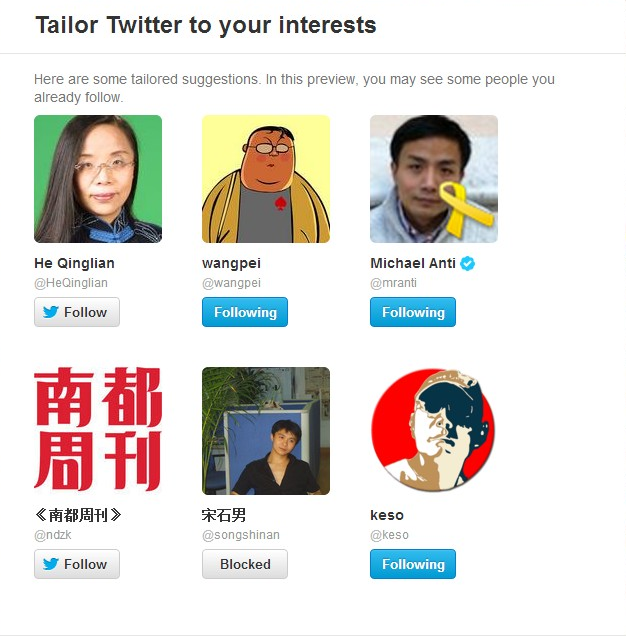
\includegraphics[width=0.9\columnwidth]{tailored}
\end{center}
\caption{Screen shot of Twitter tailored suggestion preview block}
\label{fig:tailored}
\end{figure}


Currently, Twitter does not implement this feature for profitable purpose, but they clearly states that they will do so in the future~\cite{twitterfaq}. They also indicate that they would not release these tracking data to any third party.

\section{Experiment} \label{sec:experiment}

We did a series of experiments to measure the server compliance on Do Not Track. The methodology is similar to Lorrie \emph{et al} study, with certain adjustment and enhancement compared to their experiment. We also adjust our experiment during the study and reproduce the experiment a few times. The result of the experiment is presented in the last of this section.

Our main experiment is on Twitter. We also do some supplementary experiments on Google text ads and the AdRoll and AddThis mention in Section~\ref{sec:services}. We discuss about the main experiment on Twitter in Section ~\ref{sec:pre}, ~\ref{sec:method}, ~\ref{sec:expect}, and ~\ref{sec:result}. We present those supplementary experiments in Section ~\ref{sec:supplement}. 

\subsection{Assumptions and Preparation} \label{sec:pre}

Twitter has multiple type of suggestions, including promotion suggestion, suggestion based on current Twitter network, and tailored suggestion. Twitter only claimed their support to Do Not Track on tailored suggestion. Thus we measure compliance of Twitter on Do Not Track based on tailored suggestion feature.

We select to examine Twitter tailored suggestion on Twitter tailored suggestion preview page~\cite{twittertailoredpreview}. The preview page, which is supposed to present a sample of the whole suggestion pool, could show up to six suggested accounts on each visit. It could be refreshed and the accounts showed would be shuffled. We choose this page since it is the easiest way to deduce the whole suggestion pool in Twitter server, since the suggestion block on homepage of twitter only shows up to three suggestions. These suggestions does not guarantee to contain tailored suggestions for each visit.

In the following experiment, we assume Twitter tailored suggestion preview page~\cite{twittertailoredpreview} keep strict consistency with Twitter tailored suggestion feature. I.e., the preview page, which can show up to six suggestions on each visit, would not contains any suggested accounts that are not contained in tailored suggestion account pool. Furthermore, if the preview page does not show any suggestions, the tailored suggestion pool is also empty.

We also assume that tailored suggestion is solely based on third-party tracking technology by Twitter, according to Twitter's explanation of tailored suggestion feature~\cite{twitterts}. We assume that if the user is not tracked, then there will be not any suggestions not only in the preview page showed to the user, but also in the back-end suggestion pool for this user specifically. 

When a user visits the preview page of tailored suggestion, if there is no suggestions, it will show a non-suggestion page as Figure~\ref{fig:nosug}.

We also found that tailored suggestion will not show up or changed until about three days after a new user has been registered or browsing convention has been change. Thus, we have to wait three days to obtain the correct suggestions. In this three days, we keep browsing history clean.

\begin{figure}
\begin{center}
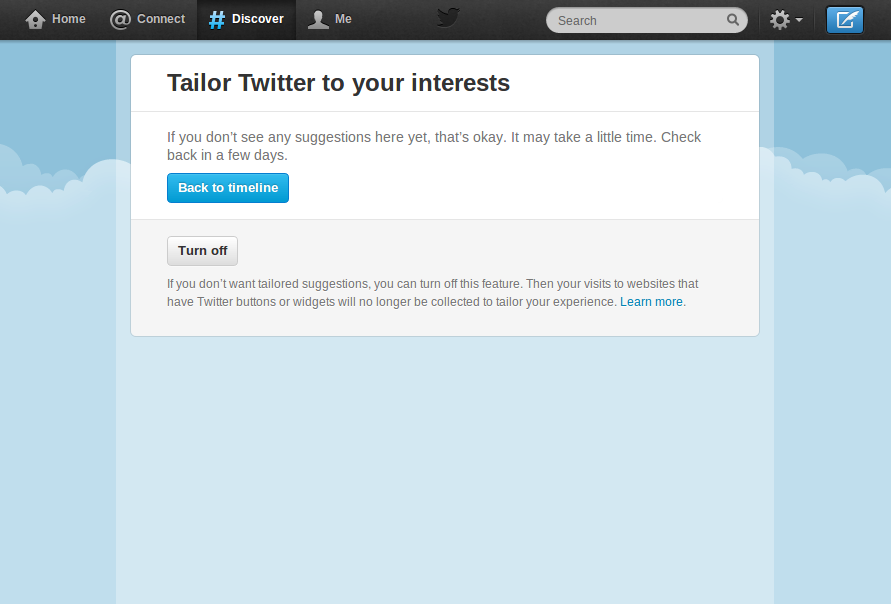
\includegraphics[width=0.9\columnwidth]{nosug}
\end{center}
\caption{Screen shot of Twitter tailored suggestion preview page with no suggestions}
\label{fig:nosug}
\end{figure}

\subsection{Methodology} \label{sec:method}

We create 4 testing Twitter accounts, make them as verified users by confirming 4 testing email accounts, and let each of them follow 10 identical accounts. These accounts are randomly selected by hand in the recommendation page, but are the same for those 4 testing accounts. These accounts are mostly celebrities such as Justin Bieber and Barack Obama. We do so because we would like to simulate the real Twitter users at most level. Due to some previous experiments we made, we found that unverified new users with 0 following accounts might not be selected as the tailored suggestion target. Also, we would like to make sure that the 4 testing accounts share the same variables for every aspects except for Do Not Track property. Of course, we enabled tailored suggestion for all accounts when registering.

For those 4 testing accounts, we differentiate them in the different ways presented in Table~\ref{table:testaccount}. The basic idea is to test:
\begin{itemize}
\item Behavior of Twitter tailored suggestion when a user expressed Do Not Track during browsing websites in Twitter ecosystem.
\item Behavior of Twitter tailored suggestion when a user does not express Do Not Track during browsing websites in Twitter ecosystem.
\item Behavior of Twitter tailored suggestion when a user expressed Do Not Track during browsing websites in Twitter ecosystem but does not expressed Do Not Track when visiting tailored suggestion preview page.

\end{itemize} 

\begin{table*}
\centering
\footnotesize
\begin{tabular}{ccccc}
\toprule
Account&Training with DNT&Training without DNT&Preview with DNT&Preview without DNT\\
\midrule
tester 1&&\checkmark&&\checkmark\\
\addlinespace
tester 2&\checkmark&&\checkmark&\\
\addlinespace
tester 3&\checkmark&&&\checkmark\\
\addlinespace
tester 4&&&&\checkmark\\
\bottomrule
\end{tabular}
\caption{Different behaviors of different testing accounts in the experiment on Twitter}
\label{table:testaccount}
\end{table*}

We would train tester 1, 2, and 3 to browsing multiple websites on a specific topic. Specifically, we use Selinum 2 with Java to generate a browser automation program that search the topic on Google.com, click all the result links on first 10 pages. This is about 100 pages. We would assume a certain portion of these websites are in Twitter ecosystem. Then we wait for a period of time to allow server update its data, and then visit and take a screen shot of the Twitter tailored suggestion preview page. The algorithm is presented in Algorithm~\ref{dntexperiment}.

\begin{algorithm}
\caption{Detect DNT friendly websites}\label{dntexperiment}
\begin{algorithmic}
\State $\text{login Twitter}$
\State $\text{Google search of the topic word}$
\State $url_list := \text{result links in first 10 pages}$
\ForAll {$url \in url_list$}
  \State $\text{visit the page of } url$
  \State $\text{, wait until the page loaded completely}$
\EndFor
\State $\text{visit Twitter tailored suggestion preview page}$
\State $\text{take a screen shot}$
\State $\text{}$
\end{algorithmic}
\end{algorithm}


We then will measure the similarity of the accounts showed up in preview page with the original top. We do this procedure by hand with our best knowledge. Admittedly this is not the most strict and precise way, but it is reasonable since the account name is very short, thus the comparison based on \emph{Cosine Similarity} used by Lorrie \emph{et al} study~\cite{balebako2012measuring} is not very applicable in our study. Since tailored suggestions would be either existed or not existed by our assumption mentioned in Section~\ref{sec:pre}, the similarity itself is not as sensitive as in Lorrie \emph{et al} study. In addition, the suggestions are mostly public well-known Twitter accounts with large population of followers. The accuracy of our examination on the similarity would be increased by this factor.

Tester 1 is a control tester that will generate browsing history and visit the preview page with Do Not Track off. Tester 2 and 3 are experimental testers: they will generate browsing history with Do Not Track on but visit the preview page with Do Not Track on and off respectively. Tester 4 is also a control tester with no browsing history and will visit the preview page directly.

To prevent our experiment being affected by tracking based on browser, rather than on user specific, we create 4 different browser profiles for each tester and keep the tester with their own profile. We select our topic as \emph{Java development}.

\subsection{Expectation} \label{sec:expect}

Regardless of Twitter's compliance of Do Not Track, tailored suggestions for tester 1 should always be related to the topic. Also, there should not be any tailored suggestion for tester 4.

If Twitter complies Do Not Track on server-side strictly, we expect there is not any tailored suggestions for tester 2 and 3. In contrast, if Twitter does not complies Do Not Track at all, there would be tailored suggestions for tester 2 and 3, and also the suggested accounts should be related to the browsing history.

There might be a third situation, that Twitter complies Do Not Track in a special way on the preview page only. Specifically, it would not show the tailored suggestions if it detected Do Not Track is on, but it still tracked the user in its server and keep the user specific data in database. For this condition, we expect that there is no suggestions for tester 2 but there will be suggestions related to the browsing history for tester 3.

\subsection{Result} \label{sec:result}

In our experiment, the tailored suggestions for tester 1 is showed in the preview page. The screen shot if showed in Figure~\ref{fig:twitter}The accounts suggested by tailored suggestion, including \emph{Google Developer, Microsoft Research, Computer Science}, etc. are closely related to the topic \emph{Java development}. 

There are no tailored suggestions showed in the preview pages for tester 2, 3, and 4. For tester 2, the preview page shows up a special text description to indicate that Do Not Track is enable when visiting this page, where the screen shot is showed in Figure~\ref{fig:dnton}

We could infer that tester 2 and 3, who browsing the websites with Do Not Track enabled, is not tracked by Twitter as a third party.

This result is consistent with the promise of Twitter. Based on our experiment, Twitter is strictly following Do Not Track standard with strong compliance.
\begin{figure}
\begin{center}
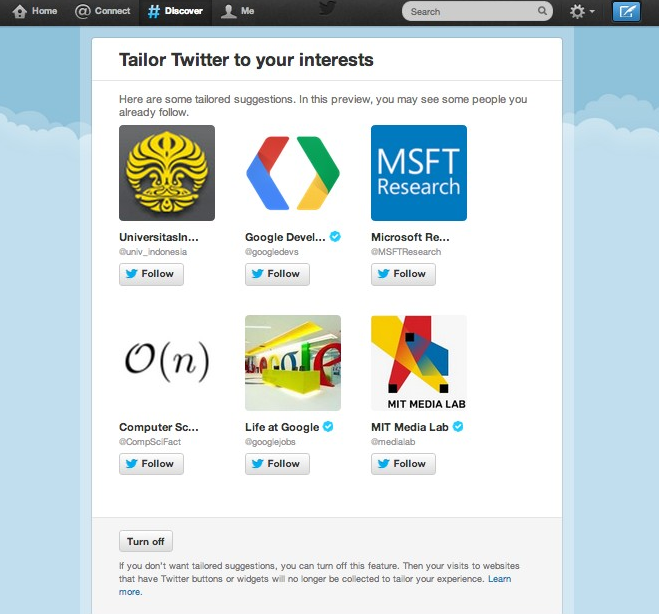
\includegraphics[width=0.9\columnwidth]{twitter}
\end{center}
\caption{Screen shot of Twitter tailored suggestion preview page of tester 1, with DNT off}
\label{fig:twitter}
\end{figure}

\begin{figure}
\begin{center}
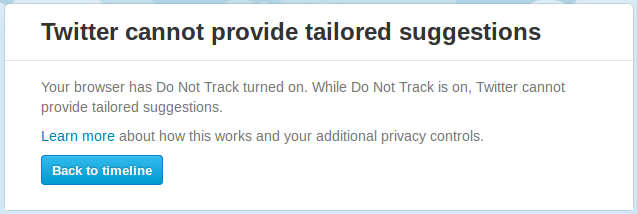
\includegraphics[width=0.9\columnwidth]{dnton}
\end{center}
\caption{Screen shot of Twitter tailored suggestion preview page with DNT on}
\label{fig:dnton}
\end{figure}

\subsection{Supplementary Experiments} \label{sec:supplement}
Along with the main experiment targeting on Twitter, we did several supplementary experiments to explore more on the compliance of Do Not Track.

\subsubsection{Twitter}
After found that Twitter is strictly respecting Do Not Track, we are wondering how Twitter will process the previous user tracking data if it detected that Do Not Track is included in user's request. We add a tester 5, who will re-do the procedure identically with tester 1. There will be relevant suggestions to browsing histories. Now we turn Do Not Track on and revisit the preview page, within expect, it shows the block as Figure\ref{fig:dnton} to indicate that Do Not Track on. Finally, we turn Do Not Track off and revisit the preview page. Surprisingly, there is no suggestions showed up, where a block as Figure\ref{fig:nosug} is displayed. 

We can, then, infer that Twitter would delete, or deprecate, the user tracking data in its back-end database. This feature is not required by Do Not Track, but is intuitive and could protect user privacy better.

\subsubsection{AdRoll and AddThis}

In Section~\ref{sec:dntheadertest}, we mentioned that we captured two URLs which echoed \verb|DNT: 1| header back. Those two URLs are \url{http://cf.addthis.com/red/p.json} and \url{https://d.adroll.com/cm/f/out}, which belongs to AddThis, a sharing data platform and AdRoll, an advertisement platform. We discussed in Section~\ref{sec:dntheadertest} that we are not able to identify where AdRoll is placing their advertisements or which web service that AddThis provide the user data to. However, we can still analysis their behavior by sending HTTP requests to them with Do Not Track on and off.

\paragraph{AdRoll}
With Do Not Track off, HTTP respond from \url{https://d.adroll.com/cm/f/out} contains:
\begin{verbatim}
HTTP/1.1 200 OK
Server: nginx/1.0.10
Date: Mon, 06 May 2013 14:51:40 GMT
Content-Type: image/gif
Connection: keep-alive
Set-Cookie: __adroll=5302ee6440dfb9467aa174d7917d9fa6; 
Version=1; Expires=Fri, 01-Jan-2021 00:00:00 GMT; 
Max-Age=432000000; Path=/
Pragma: no-cache
p3p: CP="NON DSP COR CURa PSA PSD OUR BUS NAV STA"
Content-Length: 35
Cache-Control: no-store, no-cache, must-revalidate
\end{verbatim}
in header field. As we can see, it writes cookie which will expire very long time later. This 2 by 2 all black element will not cause any attention by visitors, but might be able to track users without their notice.

With Do Not Track on, HTTP respond from \url{https://d.adroll.com/cm/f/out} contains:
\begin{verbatim}
HTTP/1.1 200 OK
Server: nginx/1.0.10
Date: Mon, 06 May 2013 14:58:16 GMT
Content-Type: image/gif
Connection: keep-alive
Set-Cookie: __adroll=expire; Version=1; Expires=Sat,
 01-Jan-2000 00:00:00 GMT; Max-Age=-100000; Path=/
Pragma: no-cache
p3p: CP="NON DSP COR CURa PSA PSD OUR BUS NAV STA"
DNT: 1
Content-Length: 35
Cache-Control: no-store, no-cache, must-revalidate
\end{verbatim}
in header field. It sets cookie, which it wrote in the request when Do Not Track off, to \verb|expire|, and set the expire date of this cookie is sometime already passed. I.e., it makes the cookie expired. We can reasonable speculate that this request does not track the user anymore.

\paragraph{AddThis}
Response obtained when sending requests to from \url{http://cf.addthis.com/red/p.json} does not involve any cookie reading or setting. However it is quite interesting that the json file it returned.

With Do Not Track on, it will return a json file contains three json object with names:

\begin{itemize}
\item \verb|"urls"|
\item \verb|"segments"|
\item \verb|"loc"|
\end{itemize}

\verb|"urls"| contains several URL strings. These could be which advertisement the user has been viewed, since the URLs are with domain of \emph{media6degrees}, \emph{addthis}, \emph{adadviser}, which are all advertisement platforms. Or it could be meaning differently. \verb|"loc"| contains a base64 encoded string: \verb|MTUyMDFOQVVTUEEyMjA0MTAwMDUwODYyODAwVg==|. It could be decoded to \verb|15201NAUSPA2204100050862800V|. This certainly contains a geolocation information since the we are located in the area of Pittsburgh, PA, USA with the zip code of 15213, which is pretty close of the area of zip code 15201. That string contains several matching information such as \textbf{15201}, \textbf{US}, \textbf{PA}. It is reasonable to speculate that this \verb|"loc"| field contains the geolocation of the user. It might not be the currently geolocation, but might be the geolocation obtained recently. \verb|"segments"| only contains an empty array.

With Do Not Track off, the jason file returned still contains \verb|"url"| and \verb|"segments"| json objects, but both of them contain an empty array. \verb|"loc"| json object is not contained in this returned json file.

\paragraph{Conclusion}

Since we can only test these two networks as a normal user with no privileges or knowledges of the server design, we can only make educational inference based on the HTTP response we received. It is reasonable to conclude that both these two URLs of AdRoll and AddThis would track users with Do Not Track off. However, both of them will stop track users when Do Not Track is enabled. Thus, AdRoll and AddThis are complying with Do Not Track. Although they do not include any detail on their privacy policies, but they expressed their supporting of Do Not Track by echoing back \verb|DNT :1| header to users.

\subsubsection{Google Text ads}
Since Lorrie \emph{et al} study~\cite{balebako2012measuring} mentions that Google will support Do Not Track in later 2012. Up to date, which is in 2013, we would like to partially reproduce the same experiment made by Lorrie \emph{et al}. We would like to modify the experiment to a easier methodology, but with less restrict logic. We would browsing websites of related topics listed by Google search on the top 10 pages, which is similar to our main experiment. We would like to compare the similarity manually by our best knowledge. We did this because we are merely to obtaining a updated result of wither Google text ads is supporting Do Not Track, rather than re-design the whole experiment with other privacy tools. Also, this is only one of our supplementary experiment.

We choose the topic as "european travel" and re-use the target website \url{chicagotribune.com/news/local/breaking} provided by the original experiment. We choose only one target site since we assume that Google text ads block embedded within different target websites behave in same way. We create 3 testers. Tester 1 and 2 will generate browsing history with Do Not Track on and off respectively. Tester 3 will not generate browsing history.

We found that tester 1, which with Do Not Track on, is still receiving Google text ads related to "european travel". The screen shot of the Google text ads block on \url{chicagotribune.com/news/local/breaking} is presented in Figure~\ref{fig:textad}. A very similar text ad is showed for tester 2. Both of them are determined to be related to the topic "european travel". A different Google text ad block, presented in Figure~\ref{fig:textadrandom} is shown to tester 3, without any browsing history. This ad block is not relevant to the topic.

Thus, we could infer that tester 1 and 2 are tracked, even tester 1 expresses Do Not Track in each HTTP requests. Thus, it can be concluded that Google text ad does not support Do Not Track yet.
\begin{figure}
\begin{center}
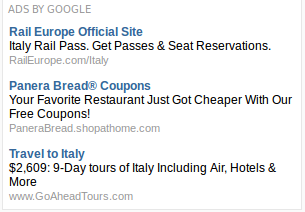
\includegraphics[width=0.9\columnwidth]{textad}
\end{center}
\caption{Screen shot of Google text ads showed to test 1 with DNT on}
\label{fig:textad}
\end{figure}

\begin{figure}
\begin{center}

\includegraphics[width=0.9\columnwidth]{textadrandom}
\end{center}
\caption{Screen shot of Google text ads showed to test 3 without browsing history}
\label{fig:textadrandom}
\end{figure}

\section{Limitation} \label{sec:limitation}


The value of this paper is not only the measurement itself, but also several limitations we discovered during our study. Some of these limitations are on the design of the Do Not Track concept; others are on the experiment methodology and implement. There is also a limitation of reality and context of the research study.

\subsection{Do Not Show or Do Not Track}

This limitation/issue exists for all studies that want to test any tool for limiting behavior advertising with any third-party entity. As stated in the DNT draft~\cite{dntdraft}, DNT requires the third-party to stop tracking by cease collection, retention, and use of all data related to the request and response. But this requirement is very hard to test in practice. 

Since most third-party company does not publish their method/algorithm regarding DNT or other tools, we can only make speculation of server’s actually behavior based on the content we are shown. For example, we may conclude that a website is compliant with the DNT protocol because they stopped showing us advertisement related to our browsing history after DNT is set to 1. However, without looking at the specific implementation of the server, we can never be sure what the server does when it sees a DNT header in the request. A server could simply keep tracking the user but instead not show the targeted ad to the user and keep the tracked browsing history data for later or other use. As a tester on the user’s end, we can not tell the difference between a server who stop collecting the data and a server who keeps collecting the data without showing the targeted ads. 


\subsection{Complexity of the online advertising ecosystem} \label{sec:complexity}
As discussed in Section~\ref{sec:dntheadertest}, the current state of advertising companies makes it hard to find out the exact websites that the advertising companies place their ad on to do any targeted test. Furthermore, the complexity of the overall Internet advertising ecosystem makes it hard to locate the tracker and do any test in isolate. 

\subsection{Immaturity of DNT standard}
The DNT proposal still need time and work to mature. At the current state, there no clear standard of the DNT specification and may websites behave differently when presented with a DNT HTTP header. This may change in a few years when the DNT specification is more extensive and the advertising industry agree on a standard way to handle DNT headers. The current DNT proposal present the following issues that hinders out test and also the implementation of servers that want to support DNT:

1. The HTTP response with DNT echo:
The 2011 March draft recommend the third party server comply by echoing a DNT header back in the HTTP response. This led us to do the experiment in Section~\ref{sec:dntheadertest}. However this recommendation is removed in all 4 subsequent publications of the specification~\cite{tracking_dnt20130430, tracking_dnt20121002, tracking_dnt20120313, tracking_dnt20111114} suggesting that the recommendation was not adopted. So there is definitely gaps between the most up to date DNT specification and the current implementation by the websites since the test we did in Section~\ref{sec:dntheadertest} shows that there are at least still a couple of websites/companies that still echo DNT:1 back. 

2. DNT Tk header with TSV
  All DNT specification following the March 2011 one talks about a Tracking Status Value(TSV) which represent the third-party server’s compliance. The TSV is supposedly sent through HTTP response with the header Tk. However, we did the tests similar to the one on Section~\ref{sec:dntheadertest} and have found that no server sent a HTTP response Tk header. This suggest the feature is still in draft stage and have not gained any support on servers. 


\section{Conclusion} \label{sec:conclusion}
\todo{add conclusion}

\section*{Acknowledgements}

We would like to specially thank Rebecca Balebako, Blase Ur and Aleecia M. McDonald for their time on providing supports and feedbacks to through our research project. We would also thank Collin Jackson, Lin-Shung Huang and Eric Chen for their guidance and useful insights. We would finally thank everyone in the public tracking team of W3C for helping us on solving problems.
\bibliographystyle{abbrv}
\bibliography{css}
\end{document}
